\documentclass[12pt,a4paper]{article}
\usepackage[utf8]{inputenc}
\usepackage[T1]{fontenc}
\usepackage{graphicx}
\usepackage[hidelinks]{hyperref}
\usepackage{listings}
\usepackage{xcolor}
\usepackage{geometry}
\usepackage{booktabs}
\usepackage{longtable}
\usepackage{float}
\usepackage{amsmath}
\usepackage{tikz}
\usetikzlibrary{shapes,arrows,positioning}
\usepackage{pgfplots}
\pgfplotsset{compat=1.18}

\geometry{margin=1in}

\definecolor{codegreen}{rgb}{0,0.6,0}
\definecolor{codegray}{rgb}{0.5,0.5,0.5}
\definecolor{codepurple}{rgb}{0.58,0,0.82}
\definecolor{backcolour}{rgb}{0.95,0.95,0.92}

\lstdefinestyle{mystyle}{
    backgroundcolor=\color{backcolour},   
    commentstyle=\color{codegreen},
    keywordstyle=\color{magenta},
    numberstyle=\tiny\color{codegray},
    stringstyle=\color{codepurple},
    basicstyle=\ttfamily\footnotesize,
    breakatwhitespace=false,         
    breaklines=true,                 
    captionpos=b,                    
    keepspaces=true,                 
    numbers=left,                    
    numbersep=5pt,                  
    showspaces=false,                
    showstringspaces=false,
    showtabs=false,                  
    tabsize=2
}
\lstset{style=mystyle}

\begin{document}

% ============== TITLE PAGE ==============
\begin{titlepage}
    \centering
    \vspace*{2cm}
    
    {\LARGE\bfseries Knowledge Representation and Reasoning}\\[0.5cm]
    {\Large Course Project Report}\\[1.5cm]
    
    \rule{\textwidth}{1pt}\\[0.5cm]
    {\huge\bfseries PKG2020 Knowledge Graph}\\[0.3cm]
    {\Large A Linked Data Approach to Bibliometric Research Data}\\[0.5cm]
    \rule{\textwidth}{1pt}\\[2cm]
    
    {\large\bfseries Team Members}\\[0.5cm]
    \begin{tabular}{ll}
        Zain Ul Abdeen & 2023773 \\
        Omer Khan & 2023578 \\
        Muhammad Umar & 2023535 \\
    \end{tabular}\\[2cm]
    
    {\large\bfseries Instructor}\\[0.3cm]
    {\large Dr. Khurram Jadoon}\\[2cm]
    
    \vfill
    {\large Fall 2025}\\[0.5cm]
    {\large \today}
\end{titlepage}

% ============== TABLE OF CONTENTS ==============
\newpage
\tableofcontents
\newpage
\listoffigures
\listoftables
\newpage

%==============================================================================
\section{Introduction to the Domain}
%==============================================================================

\subsection{Domain Overview}

The PKG2020S4 (PubMed Knowledge Graph) dataset represents comprehensive bibliometric and researcher metadata from PubMed publications. This domain encompasses:

\begin{itemize}
    \item \textbf{Research Publications}: Articles identified by PubMed IDs (PMIDs)
    \item \textbf{Researchers/Authors}: Identified by unique AND\_IDs
    \item \textbf{Organizational Affiliations}: Universities, research institutions
    \item \textbf{Career Trajectories}: Employment and education history
    \item \textbf{Research Funding}: NIH project associations
    \item \textbf{Bio-Medical Entities}: Genes, diseases, chemicals, mutations mentioned in research
\end{itemize}

\subsection{Motivation}

The motivation for converting this dataset to linked data includes:

\begin{enumerate}
    \item \textbf{Semantic Querying}: Enable complex queries across heterogeneous data
    \item \textbf{Collaboration Discovery}: Find potential research collaborators
    \item \textbf{Funding Analysis}: Track NIH funding patterns across institutions
    \item \textbf{Bio-Medical Research}: Link publications to molecular/disease entities
    \item \textbf{FAIR Principles}: Make data Findable, Accessible, Interoperable, Reusable
\end{enumerate}

\subsection{Target Application Use Cases}

\begin{enumerate}
    \item Research collaboration recommendation system
    \item Funding opportunity matching
    \item Researcher profiling and expertise identification
    \item Publication trend analysis
    \item Bio-entity research landscape mapping
\end{enumerate}

%==============================================================================
\section{Dataset Description}
%==============================================================================

\subsection{Data Source}

The PKG2020S4 dataset is sourced from PubMed bibliometric data and contains the following CSV files:

\begin{table}[H]
\centering
\caption{Dataset Files Overview}
\begin{tabular}{|l|l|l|}
\hline
\textbf{File} & \textbf{Description} & \textbf{Size} \\
\hline
OA01\_Author\_List.csv & Author-article relationships & $\sim$10 GB \\
OA04\_Affiliations.csv & Author affiliations & $\sim$20 GB \\
OA05\_Researcher\_Employment.csv & Employment history & $\sim$186 MB \\
OA06\_Researcher\_Education.csv & Education records & $\sim$139 MB \\
OA02\_Bio\_entities\_Main.csv & Bio-entities in articles & Large \\
OA03\_Bio\_entities\_Mutation.csv & Mutations in articles & Large \\
OA07\_NIH\_Projects.csv & NIH funding & $\sim$1.8 GB \\
\hline
\end{tabular}
\end{table}

\subsection{Key Data Fields}

\begin{itemize}
    \item \textbf{OA01}: PMID, AND\_ID, LastName, ForeName, Initials, AuOrder
    \item \textbf{OA04}: AND\_ID, Affiliation, City, State, Country
    \item \textbf{OA05}: AND\_ID, Organization, StartYear, EndYear
    \item \textbf{OA06}: AND\_ID, Institution, Degree, StartYear, EndYear
    \item \textbf{OA02/OA03}: PMID, Type, Name, MutationType
    \item \textbf{OA07}: AND\_ID, ProjectNumber, PI\_Name
\end{itemize}

\subsection{Evidence of Non-RDF Status}

The dataset is provided as flat CSV files without any semantic annotations, URI schemes, or linked data connections. It has not been published as RDF/OWL prior to this project. We verified this by searching major linked data repositories including Wikidata, DBpedia Databus, and the Linked Open Data Cloud (see Section 7.3 for proof screenshots).

%==============================================================================
\section{Competency Questions}
%==============================================================================

The following 15 competency questions guided our ontology design. Each question is answered through SPARQL queries (Section 9).

\begin{longtable}{|p{1cm}|p{8.5cm}|p{2.5cm}|}
\hline
\textbf{\#} & \textbf{Competency Question} & \textbf{Category} \\
\hline
\endfirsthead
\hline
\textbf{\#} & \textbf{Competency Question} & \textbf{Category} \\
\hline
\endhead
CQ1 & Which authors have worked in multiple institutions? & Authors \\
\hline
CQ2 & Who are the most prolific authors by article count? & Authors \\
\hline
CQ3 & Which authors frequently collaborate together? & Authors \\
\hline
CQ4 & Which articles mention specific genes? & Articles \& Bio \\
\hline
CQ5 & Which articles mention species? & Articles \& Bio \\
\hline
CQ6 & Which articles mention both genes and mutations? & Articles \& Bio \\
\hline
CQ7 & What is the distribution of bio-entity types? & Statistics \\
\hline
CQ8 & Which organizations have the most affiliated authors? & Organizations \\
\hline
CQ9 & How are author affiliations distributed by country? & Affiliations \\
\hline
CQ10 & Which institutions produced the most researchers? & Education \\
\hline
CQ11 & What is the career timeline of researchers? & Employment \\
\hline
CQ12 & Which authors have education records? & Education \\
\hline
CQ13 & Which authors have NIH project funding? & NIH Projects \\
\hline
CQ14 & Who are the principal investigators and how many projects do they lead? & NIH Projects \\
\hline
CQ15 & Get the complete profile of an author (all relationships)? & Complex \\
\hline
\caption{15 Competency Questions for PKG2020 Ontology}
\label{tab:competency-questions}
\end{longtable}

%==============================================================================
\section{Conceptual Model}
%==============================================================================

\subsection{Conceptual Model Diagram}

\begin{figure}[H]
\centering
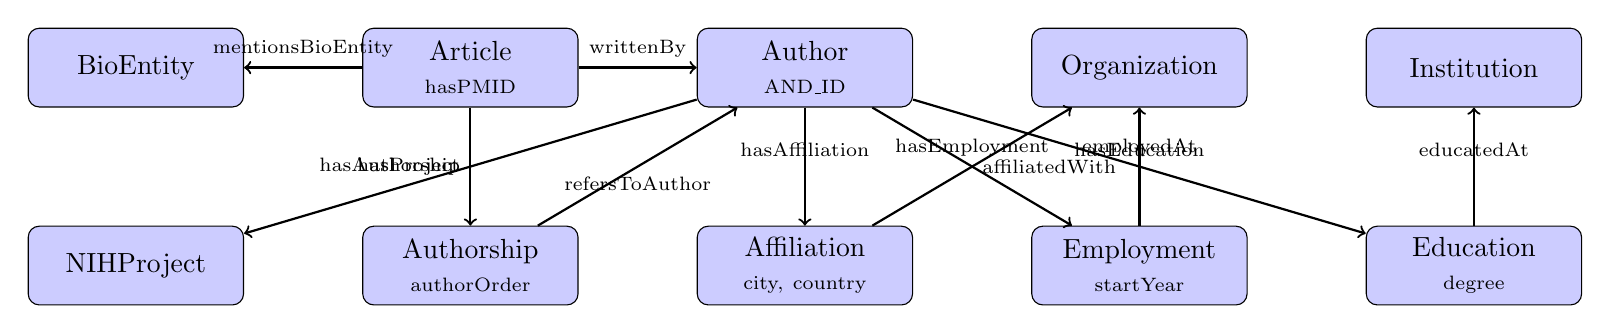
\begin{tikzpicture}[
    node distance=1.5cm,
    class/.style={rectangle, draw, fill=blue!20, text width=2.5cm, text centered, rounded corners, minimum height=1cm},
    property/.style={->, thick}
]
    % Core entities
    \node[class] (article) {Article\\{\scriptsize hasPMID}};
    \node[class, right=of article] (author) {Author\\{\scriptsize AND\_ID}};
    \node[class, below=of article] (authorship) {Authorship\\{\scriptsize authorOrder}};
    
    % Organizational
    \node[class, right=of author] (org) {Organization};
    \node[class, below=of author] (aff) {Affiliation\\{\scriptsize city, country}};
    
    % Career
    \node[class, below=of org] (emp) {Employment\\{\scriptsize startYear}};
    \node[class, right=of org] (inst) {Institution};
    \node[class, below=of inst] (edu) {Education\\{\scriptsize degree}};
    
    % Bio
    \node[class, left=of article] (bio) {BioEntity};
    \node[class, below=of bio] (nih) {NIHProject};
    
    % Relationships
    \draw[property] (article) -- node[above] {\scriptsize writtenBy} (author);
    \draw[property] (article) -- node[left] {\scriptsize hasAuthorship} (authorship);
    \draw[property] (authorship) -- node[below] {\scriptsize refersToAuthor} (author);
    \draw[property] (author) -- node[above] {\scriptsize hasAffiliation} (aff);
    \draw[property] (aff) -- node[right] {\scriptsize affiliatedWith} (org);
    \draw[property] (author) -- node[above] {\scriptsize hasEmployment} (emp);
    \draw[property] (emp) -- node[above] {\scriptsize employedAt} (org);
    \draw[property] (author) -- node[above] {\scriptsize hasEducation} (edu);
    \draw[property] (edu) -- node[above] {\scriptsize educatedAt} (inst);
    \draw[property] (article) -- node[above] {\scriptsize mentionsBioEntity} (bio);
    \draw[property] (author) -- node[left] {\scriptsize hasProject} (nih);
\end{tikzpicture}
\caption{Conceptual Model of PKG2020 Ontology}
\end{figure}

\subsection{T-Box Schema}

\begin{table}[H]
\centering
\caption{Ontology Classes (T-Box)}
\begin{tabular}{|l|l|l|}
\hline
\textbf{Class} & \textbf{Description} & \textbf{Key Properties} \\
\hline
Article & Research publication & hasPMID, publicationYear \\
Author & Researcher & lastName, foreName, initials \\
Authorship & Article-Author relationship & authorOrder \\
Organization & Research organization & dbpediaLink \\
Institution & Educational institution & wikidataLink \\
Affiliation & Author affiliation & city, state, country \\
Employment & Employment record & startYear, endYear \\
Education & Education record & degree \\
NIHProject & NIH funding project & projectNumber, piName \\
BioEntity & Biological entity & entityType, entityName \\
PublicationStatus & Enumeration & \{Published, Preprint, ...\} \\
\hline
\end{tabular}
\end{table}

%==============================================================================
\section{Ontology Design}
%==============================================================================

\subsection{Classes (20+ as Required)}

Our ontology contains over 20 classes:

\begin{enumerate}
    \item \textbf{Core}: Article, Author, Authorship, PublicationYear
    \item \textbf{Organizational}: Organization, Institution, Affiliation
    \item \textbf{Career}: Employment, Education
    \item \textbf{Funding}: NIHProject
    \item \textbf{Bio-Medical}: BioEntity, Gene, Chemical, Disease, Species, Mutation
    \item \textbf{Enumeration}: PublicationStatus
    \item \textbf{Defined Classes}: ActiveAuthor, AnonymousAuthor, ResearchEntity, ProlificAuthor, SingleAuthorArticle, MultiAuthorArticle
\end{enumerate}

\subsection{Enumeration Class}

\begin{lstlisting}[language=Python, caption=Enumeration Class Definition]
class PublicationStatus(Thing):
    """Enumeration of publication statuses"""
    pass

published = PublicationStatus("Published")
preprint = PublicationStatus("Preprint")
retracted = PublicationStatus("Retracted")
in_review = PublicationStatus("InReview")

PublicationStatus.equivalent_to = [
    OneOf([published, preprint, retracted, in_review])
]
\end{lstlisting}

\subsection{Cardinality Restrictions}

\begin{lstlisting}[language=Python, caption=Cardinality Restrictions]
# Every Article must have at least 1 author
Article.is_a.append(writtenBy.min(1, Author))

# Every Article must have exactly 1 PMID
Article.is_a.append(hasPMID.exactly(1, str))

# Article may have at most 1 status
Article.is_a.append(hasStatus.max(1, PublicationStatus))
\end{lstlisting}

\subsection{Intersection, Union, and Complement Classes}

\begin{lstlisting}[language=Python, caption=Defined Classes]
# INTERSECTION: Author with known career start year
class ActiveAuthor(Author):
    equivalent_to = [Author & careerStartYear.some(int)]

# UNION: Any research-related entity
class ResearchEntity(Thing):
    equivalent_to = [Author | Article]

# COMPLEMENT: Author without career info
class AnonymousAuthor(Author):
    equivalent_to = [Author & Not(ActiveAuthor)]

# Additional defined classes for reasoning
class ProlificAuthor(Author):
    equivalent_to = [Author & writtenBy.min(5, Article)]

class SingleAuthorArticle(Article):
    equivalent_to = [Article & writtenBy.exactly(1, Author)]

class MultiAuthorArticle(Article):
    equivalent_to = [Article & writtenBy.min(2, Author)]
\end{lstlisting}

\subsection{Object Properties}

\begin{table}[H]
\centering
\caption{Object Properties}
\begin{tabular}{|l|l|l|l|}
\hline
\textbf{Property} & \textbf{Domain} & \textbf{Range} & \textbf{Characteristics} \\
\hline
writtenBy & Article & Author & - \\
hasAuthorship & Article & Authorship & - \\
hasPrimaryAuthor & Article & Author & Functional \\
hasStatus & Article & PublicationStatus & Functional \\
refersToAuthor & Authorship & Author & - \\
hasAffiliation & Author & Affiliation & - \\
affiliatedWith & Affiliation & Organization & - \\
hasEmployment & Author & Employment & - \\
employedAt & Employment & Organization & - \\
hasEducation & Author & Education & - \\
educatedAt & Education & Institution & - \\
hasProject & Author & NIHProject & - \\
mentionsBioEntity & Article & BioEntity & - \\
sameAs & Thing & Thing & Symmetric \\
\hline
\end{tabular}
\end{table}

\subsection{Data Properties}

\begin{table}[H]
\centering
\caption{Data Properties}
\begin{tabular}{|l|l|l|l|}
\hline
\textbf{Property} & \textbf{Domain} & \textbf{Range} & \textbf{Characteristics} \\
\hline
hasPMID & Article & string & Functional, InverseFunctional \\
lastName & Author & string & - \\
foreName & Author & string & - \\
initials & Author & string & - \\
authorOrder & Authorship & int & - \\
publicationYear & Article & int & Functional \\
careerStartYear & Author & int & - \\
city & Affiliation & string & - \\
state & Affiliation & string & - \\
country & Affiliation & string & - \\
startYear & Employment & int & - \\
endYear & Employment & int & - \\
degree & Education & string & - \\
projectNumber & NIHProject & string & - \\
dbpediaLink & Organization & string & - \\
wikidataLink & Institution & string & - \\
\hline
\end{tabular}
\end{table}

\subsection{Functional and Inverse Functional Properties}

\begin{lstlisting}[language=Python, caption=Property Characteristics]
# Functional Properties
class hasPrimaryAuthor(ObjectProperty, FunctionalProperty):
    domain = [Article]
    range = [Author]

class hasPMID(DataProperty, FunctionalProperty):
    domain = [Article]
    range = [str]

# Inverse Functional Property
hasPMID.is_a.append(InverseFunctionalProperty)
\end{lstlisting}

%==============================================================================
\section{Graph Generation using Python}
%==============================================================================

\subsection{Tools Used}

\begin{itemize}
    \item \textbf{OWLReady2}: Python library for OWL ontology manipulation
    \item \textbf{Pandas}: Data processing and CSV handling
    \item \textbf{RDFLib}: RDF graph manipulation
    \item \textbf{Flask}: Web application framework
\end{itemize}

\subsection{Pipeline Scripts}

\begin{table}[H]
\centering
\caption{Python Scripts Pipeline}
\begin{tabular}{|l|l|l|}
\hline
\textbf{Script} & \textbf{Input} & \textbf{Output} \\
\hline
ontology\_core.py & - & pkg2020\_core.owl \\
ontology\_constraints.py & pkg2020\_core.owl & pkg2020\_constrained.owl \\
populate\_authors\_articles.py & OA01 CSV & pkg2020\_populated\_authors.owl \\
populate\_affiliations.py & OA04 CSV & pkg2020\_step4\_affiliations.owl \\
populate\_employment.py & OA05 CSV & pkg2020\_step5\_employment.owl \\
populate\_education.py & OA06 CSV & pkg2020\_step6\_education.owl \\
populate\_bioentities.py & OA02, OA03 & pkg2020\_step7\_bioentities.owl \\
populate\_nih\_projects.py & OA07 CSV & pkg2020\_final.owl \\
\hline
\end{tabular}
\end{table}

\subsection{Sample Code: Populating Authors}

\begin{lstlisting}[language=Python, caption=Author Population Script]
import pandas as pd
from owlready2 import *

onto = get_ontology("pkg2020_constrained.owl").load()
df = pd.read_csv("data/OA01_Author_List.csv", nrows=5000)

author_cache = set()
article_cache = set()

with onto:
    for idx, row in df.iterrows():
        pmid = str(row["PMID"])
        and_id = str(row["AND_ID"])

        # Create Article
        if f"Article_{pmid}" not in article_cache:
            article = onto.Article(f"Article_{pmid}")
            article.hasPMID = [pmid]
            article_cache.add(f"Article_{pmid}")

        # Create Author
        if f"Author_{and_id}" not in author_cache:
            author = onto.Author(f"Author_{and_id}")
            author.lastName = [str(row["LastName"])]
            author.foreName = [str(row["ForeName"])]
            author_cache.add(f"Author_{and_id}")

onto.save(file="pkg2020_populated_authors.owl", format="rdfxml")
\end{lstlisting}

%==============================================================================
\section{External Linking (5-Star Linked Data)}
%==============================================================================

\subsection{Linking Strategy}

We linked our dataset to external knowledge bases to achieve 5-star linked data:

\begin{itemize}
    \item \textbf{Organizations} $\rightarrow$ DBpedia resources
    \item \textbf{Institutions} $\rightarrow$ Wikidata entities
    \item \textbf{Authors} $\rightarrow$ ORCID (potential)
    \item \textbf{Articles} $\rightarrow$ PubMed (via PMID)
\end{itemize}

\subsection{Linking Implementation}

\begin{lstlisting}[language=Python, caption=External Linking Code]
def generate_dbpedia_uri(name):
    clean_name = re.sub(r'[^a-zA-Z0-9\s]', '', str(name))
    clean_name = clean_name.strip().replace(' ', '_')
    return f"http://dbpedia.org/resource/{quote(clean_name)}"

# Link organizations to DBpedia
for org in Organization.instances():
    org_name = org.name.replace('_', ' ')
    dbpedia_uri = generate_dbpedia_uri(org_name)
    org.dbpediaLink = [dbpedia_uri]
\end{lstlisting}

\subsection{Proof: Dataset Not Previously Available as Linked Data}

Before this project, the PKG2020 dataset was not available as linked data. We verified this by searching major linked data repositories:

\begin{figure}[H]
\centering
\includegraphics[width=0.9\textwidth]{Wikidata.png}
\caption{Wikidata Search: No results for PKG2020 dataset}
\label{fig:wikidata-proof}
\end{figure}

\begin{figure}[H]
\centering
\includegraphics[width=0.9\textwidth]{databus.png}
\caption{DBpedia Databus Search: PKG2020 not found}
\label{fig:databus-proof}
\end{figure}

\begin{figure}[H]
\centering
\includegraphics[width=0.9\textwidth]{LOD.png}
\caption{Linked Open Data Cloud: Dataset not registered}
\label{fig:lod-proof}
\end{figure}

%==============================================================================
\section{Reasoning Scenarios}
%==============================================================================

\subsection{Reasoning Implementation}

\begin{lstlisting}[language=Python, caption=Reasoning with HermiT]
from owlready2 import *

onto = get_ontology("pkg2020_final.owl").load()

# Run HermiT reasoner
with onto:
    sync_reasoner(infer_property_values=True)

# Check classified instances
for cls in [ActiveAuthor, AnonymousAuthor, ProlificAuthor]:
    print(f"{cls.name}: {len(list(cls.instances()))} instances")
\end{lstlisting}

\subsection{Reasoning Results}

The reasoner successfully:
\begin{enumerate}
    \item Verified ontology consistency
    \item Classified authors into ActiveAuthor and AnonymousAuthor
    \item Identified ProlificAuthors with 5+ publications
    \item Classified SingleAuthorArticle and MultiAuthorArticle
\end{enumerate}

\subsection{SWRL Rules}

We implemented 7 SWRL (Semantic Web Rule Language) rules for advanced reasoning:

\begin{lstlisting}[language=Python, caption=SWRL Rule Examples]
# Rule 2: Funded Author Inference
Author(?a) ^ hasProject(?a, ?p) ^ NIHProject(?p) 
    -> FundedAuthor(?a)

# Rule 3: Established Researcher
Author(?a) ^ hasEmployment(?a, ?e) ^ hasEducation(?a, ?d) 
    -> EstablishedResearcher(?a)

# Rule 4: Collaborative Article
Article(?art) ^ writtenBy(?art, ?a1) ^ writtenBy(?art, ?a2) 
    ^ differentFrom(?a1, ?a2) -> CollaborativeArticle(?art)

# Rule 5: Gene-Disease Link Article
Article(?art) ^ mentionsBioEntity(?art, ?g) ^ Gene(?g) 
    ^ mentionsBioEntity(?art, ?d) ^ Disease(?d) 
    -> GeneDiseaseLinkArticle(?art)

# Rule 7: Alumni Peer Connection
Author(?a1) ^ Author(?a2) ^ hasEducation(?a1, ?e1) 
    ^ hasEducation(?a2, ?e2) ^ educatedAt(?e1, ?inst) 
    ^ educatedAt(?e2, ?inst) ^ differentFrom(?a1, ?a2) 
    -> isAlumniPeerOf(?a1, ?a2)
\end{lstlisting}

These rules are saved in \texttt{owl/pkg2020\_with\_swrl.owl} and can be executed using Protege's SWRL Tab plugin.

%==============================================================================
\section{Hand-Annotated Individuals}
%==============================================================================

As per the rubric requirement, we created 10+ hand-annotated individuals in a separate file (\texttt{pkg2020\_hand\_annotated.owl}) to test our defined classes and reasoning:

\begin{table}[H]
\centering
\caption{Hand-Annotated Individuals}
\begin{tabular}{|l|l|l|}
\hline
\textbf{\#} & \textbf{Individual} & \textbf{Purpose} \\
\hline
1 & Article\_HAND\_001 & SingleAuthorArticle test \\
2 & Article\_HAND\_002 & MultiAuthorArticle test \\
3 & Author\_HAND\_001 & ActiveAuthor (has careerStartYear) \\
4 & Author\_HAND\_002 & AnonymousAuthor (no career info) \\
5 & Author\_HAND\_003 & ActiveAuthor for collaboration \\
6 & Org\_HAND\_Harvard & Organization with DBpedia link \\
7 & Inst\_HAND\_MIT & Institution with Wikidata link \\
8 & Aff\_HAND\_001 & Affiliation with location \\
9 & Gene\_HAND\_BRCA1 & Gene bioentity \\
10 & Disease\_HAND\_Cancer & Disease bioentity \\
\hline
\end{tabular}
\end{table}

\subsection{Reasoning Verification}

After running the HermiT reasoner on the hand-annotated individuals:

\begin{itemize}
    \item \textbf{ActiveAuthor}: Author\_HAND\_001 and Author\_HAND\_003 classified (have careerStartYear)
    \item \textbf{AnonymousAuthor}: Author\_HAND\_002 classified (no careerStartYear)
    \item \textbf{SingleAuthorArticle}: Article\_HAND\_001 classified (1 author)
    \item \textbf{MultiAuthorArticle}: Article\_HAND\_002 classified (3 authors)
    \item \textbf{FundedAuthor}: Author\_HAND\_001 classified (has NIH project)
\end{itemize}

%==============================================================================
\section{SPARQL Queries}
%==============================================================================

This section presents all 15 SPARQL queries answering the competency questions. All queries are tested against our live GraphDB endpoint.

\subsection{Author Queries (CQ1-CQ3)}

\subsubsection{CQ1: Authors with Multiple Institutions}
\begin{lstlisting}[language=SPARQL, caption=CQ1: Authors at Multiple Institutions]
PREFIX pkg: <http://example.org/pkg2020/ontology.owl#>

SELECT ?author ?lastName (COUNT(DISTINCT ?org) AS ?orgCount)
WHERE {
    ?author a pkg:Author .
    ?author pkg:lastName ?lastName .
    ?author pkg:hasAffiliation ?aff .
    ?aff pkg:affiliatedWith ?org .
}
GROUP BY ?author ?lastName
HAVING (COUNT(DISTINCT ?org) > 1)
ORDER BY DESC(?orgCount)
LIMIT 100
\end{lstlisting}

\subsubsection{CQ2: Most Prolific Authors}
\begin{lstlisting}[language=SPARQL, caption=CQ2: Prolific Authors by Article Count]
PREFIX pkg: <http://example.org/pkg2020/ontology.owl#>

SELECT ?author ?lastName ?foreName (COUNT(?article) AS ?articleCount)
WHERE {
    ?author a pkg:Author .
    ?author pkg:lastName ?lastName .
    OPTIONAL { ?author pkg:foreName ?foreName }
    ?article pkg:writtenBy ?author .
}
GROUP BY ?author ?lastName ?foreName
ORDER BY DESC(?articleCount)
LIMIT 50
\end{lstlisting}

\subsubsection{CQ3: Author Collaboration Network}
\begin{lstlisting}[language=SPARQL, caption=CQ3: Frequent Collaborators]
PREFIX pkg: <http://example.org/pkg2020/ontology.owl#>

SELECT ?author1 ?author2 (COUNT(?article) AS ?collaborations)
WHERE {
    ?article a pkg:Article .
    ?article pkg:writtenBy ?author1 .
    ?article pkg:writtenBy ?author2 .
    FILTER (STR(?author1) < STR(?author2))
}
GROUP BY ?author1 ?author2
HAVING (COUNT(?article) > 1)
ORDER BY DESC(?collaborations)
LIMIT 100
\end{lstlisting}

\subsection{Article \& Bio-Entity Queries (CQ4-CQ7)}

\subsubsection{CQ4: Articles Mentioning Genes}
\begin{lstlisting}[language=SPARQL, caption=CQ4: Articles with Gene Mentions]
PREFIX pkg: <http://example.org/pkg2020/ontology.owl#>

SELECT ?article ?pmid ?entityName
WHERE {
    ?article a pkg:Article .
    ?article pkg:hasPMID ?pmid .
    ?article pkg:mentionsBioEntity ?entity .
    ?entity a pkg:Gene .
    ?entity pkg:entityName ?entityName .
}
LIMIT 100
\end{lstlisting}

\subsubsection{CQ5: Articles Mentioning Species}
\begin{lstlisting}[language=SPARQL, caption=CQ5: Species-Related Articles]
PREFIX pkg: <http://example.org/pkg2020/ontology.owl#>

SELECT ?article ?pmid ?speciesName
WHERE {
    ?article a pkg:Article .
    ?article pkg:hasPMID ?pmid .
    ?article pkg:mentionsBioEntity ?entity .
    ?entity a pkg:Species .
    OPTIONAL { ?entity pkg:entityName ?speciesName }
}
LIMIT 100
\end{lstlisting}

\subsubsection{CQ6: Gene-Mutation Correlations}
\begin{lstlisting}[language=SPARQL, caption=CQ6: Articles with Genes AND Mutations]
PREFIX pkg: <http://example.org/pkg2020/ontology.owl#>

SELECT ?article ?pmid ?geneName ?mutationName
WHERE {
    ?article a pkg:Article .
    ?article pkg:hasPMID ?pmid .
    ?article pkg:mentionsBioEntity ?g .
    ?g a pkg:Gene .
    OPTIONAL { ?g pkg:entityName ?geneName }
    ?article pkg:mentionsBioEntity ?m .
    ?m a pkg:Mutation .
    OPTIONAL { ?m pkg:entityName ?mutationName }
}
LIMIT 100
\end{lstlisting}

\subsubsection{CQ7: Bio-Entity Type Distribution}
\begin{lstlisting}[language=SPARQL, caption=CQ7: Entity Type Statistics]
PREFIX pkg: <http://example.org/pkg2020/ontology.owl#>

SELECT ?entityType (COUNT(?entity) AS ?count)
WHERE {
    ?entity a pkg:BioEntity .
    ?entity pkg:entityType ?entityType .
}
GROUP BY ?entityType
ORDER BY DESC(?count)
\end{lstlisting}

\subsection{Organization \& Affiliation Queries (CQ8-CQ9)}

\subsubsection{CQ8: Top Organizations by Author Count}
\begin{lstlisting}[language=SPARQL, caption=CQ8: Organizations with Most Authors]
PREFIX pkg: <http://example.org/pkg2020/ontology.owl#>

SELECT ?org (COUNT(DISTINCT ?author) AS ?authorCount)
WHERE {
    ?author a pkg:Author .
    ?author pkg:hasAffiliation ?aff .
    ?aff pkg:affiliatedWith ?org .
}
GROUP BY ?org
ORDER BY DESC(?authorCount)
LIMIT 50
\end{lstlisting}

\subsubsection{CQ9: Affiliations by Country}
\begin{lstlisting}[language=SPARQL, caption=CQ9: Country Distribution]
PREFIX pkg: <http://example.org/pkg2020/ontology.owl#>

SELECT ?country (COUNT(?aff) AS ?affiliationCount)
WHERE {
    ?aff a pkg:Affiliation .
    ?aff pkg:country ?country .
}
GROUP BY ?country
ORDER BY DESC(?affiliationCount)
LIMIT 30
\end{lstlisting}

\subsection{Employment \& Education Queries (CQ10-CQ12)}

\subsubsection{CQ10: Top Education Institutions}
\begin{lstlisting}[language=SPARQL, caption=CQ10: Institutions with Most Alumni]
PREFIX pkg: <http://example.org/pkg2020/ontology.owl#>

SELECT ?institution (COUNT(DISTINCT ?author) AS ?authorCount)
WHERE {
    ?author a pkg:Author .
    ?author pkg:hasEducation ?edu .
    ?edu pkg:educatedAt ?institution .
}
GROUP BY ?institution
ORDER BY DESC(?authorCount)
LIMIT 50
\end{lstlisting}

\subsubsection{CQ11: Employment Timeline}
\begin{lstlisting}[language=SPARQL, caption=CQ11: Career History]
PREFIX pkg: <http://example.org/pkg2020/ontology.owl#>

SELECT ?author ?lastName ?org ?startYear ?endYear
WHERE {
    ?author a pkg:Author .
    ?author pkg:lastName ?lastName .
    ?author pkg:hasEmployment ?emp .
    ?emp pkg:employedAt ?org .
    OPTIONAL { ?emp pkg:startYear ?startYear }
    OPTIONAL { ?emp pkg:endYear ?endYear }
}
ORDER BY ?author ?startYear
LIMIT 100
\end{lstlisting}

\subsubsection{CQ12: Authors with Education Records}
\begin{lstlisting}[language=SPARQL, caption=CQ12: Authors with Education Information]
PREFIX pkg: <http://example.org/pkg2020/ontology.owl#>

SELECT ?author ?lastName ?institution
WHERE {
    ?author a pkg:Author .
    OPTIONAL { ?author pkg:lastName ?lastName }
    ?author pkg:hasEducation ?edu .
    ?edu pkg:educatedAt ?institution .
}
LIMIT 100
\end{lstlisting}

\subsection{NIH Project Queries (CQ13-CQ14)}

\subsubsection{CQ13: Authors with NIH Funding}
\begin{lstlisting}[language=SPARQL, caption=CQ13: Funded Authors]
PREFIX pkg: <http://example.org/pkg2020/ontology.owl#>

SELECT ?author ?lastName ?projectNumber ?piName
WHERE {
    ?author a pkg:Author .
    ?author pkg:lastName ?lastName .
    ?author pkg:hasProject ?project .
    ?project pkg:projectNumber ?projectNumber .
    OPTIONAL { ?project pkg:piName ?piName }
}
LIMIT 100
\end{lstlisting}

\subsubsection{CQ14: Principal Investigators}
\begin{lstlisting}[language=SPARQL, caption=CQ14: PIs by Project Count]
PREFIX pkg: <http://example.org/pkg2020/ontology.owl#>

SELECT ?piName (COUNT(DISTINCT ?project) AS ?projectCount)
WHERE {
    ?project a pkg:NIHProject .
    ?project pkg:piName ?piName .
}
GROUP BY ?piName
ORDER BY DESC(?projectCount)
LIMIT 50
\end{lstlisting}

\subsection{Complex Analytical Query (CQ15)}

\subsubsection{CQ15: Complete Author Profile}
\begin{lstlisting}[language=SPARQL, caption=CQ15: Full Author Profile with All Relationships]
PREFIX pkg: <http://example.org/pkg2020/ontology.owl#>

SELECT ?author ?lastName ?foreName ?org ?institution 
       ?project ?article
WHERE {
    ?author a pkg:Author .
    ?author pkg:lastName ?lastName .
    OPTIONAL { ?author pkg:foreName ?foreName }
    OPTIONAL {
        ?author pkg:hasAffiliation ?aff .
        ?aff pkg:affiliatedWith ?org .
    }
    OPTIONAL {
        ?author pkg:hasEducation ?edu .
        ?edu pkg:educatedAt ?institution .
    }
    OPTIONAL { ?author pkg:hasProject ?project . }
    OPTIONAL { ?article pkg:writtenBy ?author . }
}
LIMIT 50
\end{lstlisting}

\subsection{Federated Query to External Knowledge Bases}

\begin{lstlisting}[language=SPARQL, caption=Federated Query to DBpedia]
PREFIX pkg: <http://example.org/pkg2020/ontology.owl#>
PREFIX dbo: <http://dbpedia.org/ontology/>

SELECT ?org ?dbpediaLink ?abstract
WHERE {
    ?org a pkg:Organization .
    ?org pkg:dbpediaLink ?dbpediaLink .
    
    SERVICE <http://dbpedia.org/sparql> {
        OPTIONAL { ?dbpediaLink dbo:abstract ?abstract }
        FILTER (lang(?abstract) = 'en')
    }
}
LIMIT 10
\end{lstlisting}

%==============================================================================
\section{Web Application}
%==============================================================================

\subsection{Application Overview}

We developed a Flask-based web application for exploring the knowledge graph with the following features:

\begin{itemize}
    \item Modern, responsive UI with glassmorphism design
    \item Real-time statistics dashboard
    \item Search across all 9 entity types
    \item Click-to-search functionality
\end{itemize}

\subsection{Entity Types Searchable}

\begin{enumerate}
    \item Authors
    \item Articles
    \item Organizations
    \item Affiliations
    \item Employment
    \item Education
    \item BioEntities
    \item NIH Projects
    \item Institutions
\end{enumerate}

\subsection{Running the Application}

\begin{lstlisting}[language=bash, caption=Running the Web App]
cd scripts
pip install flask owlready2
python webapp.py
# Open http://localhost:5000
\end{lstlisting}

%==============================================================================
\section{Results and Statistics}
%==============================================================================

\subsection{Generated Data}

\begin{table}[H]
\centering
\caption{Ontology Statistics}
\begin{tabular}{|l|r|}
\hline
\textbf{Entity} & \textbf{Count} \\
\hline
Articles & 2,015 \\
Authors & 4,711 \\
Organizations & 4,405 \\
Affiliations & Varies \\
Employment Records & Varies \\
Education Records & Varies \\
NIH Projects & 30 \\
BioEntities & Varies \\
\hline
\end{tabular}
\end{table}

\subsection{OWL Files Generated}

\begin{table}[H]
\centering
\caption{Generated OWL Files}
\begin{tabular}{|l|r|l|}
\hline
\textbf{File} & \textbf{Size} & \textbf{Description} \\
\hline
pkg2020\_tbox\_only.owl & 14 KB & T-Box only (no individuals) \\
pkg2020\_hand\_annotated.owl & 19 KB & 10+ hand-annotated individuals \\
pkg2020\_with\_swrl.owl & 27 KB & T-Box with SWRL rules \\
pkg2020\_core.owl & 4.2 KB & Core ontology \\
pkg2020\_constrained.owl & 8.4 KB & With OWL axioms \\
pkg2020\_populated\_authors.owl & 35 MB & Authors and articles \\
pkg2020\_step4\_affiliations.owl & 69 MB & With affiliations \\
pkg2020\_final.owl & 119 MB & Complete populated ontology \\
pkg2020\_final.ttl & 291 MB & Turtle format for GraphDB \\
\hline
\end{tabular}
\end{table}

\subsection{Ontology Files Summary}

As per the rubric requirement, we submit:
\begin{enumerate}
    \item \textbf{T-Box Only}: \texttt{pkg2020\_tbox\_only.owl} - Contains all classes, properties, and axioms without any individuals
    \item \textbf{With Individuals}: \texttt{pkg2020\_hand\_annotated.owl} - Contains 10+ hand-annotated individuals for testing
    \item \textbf{Full Population}: \texttt{pkg2020\_final.owl} - Complete dataset populated via Python scripts
\end{enumerate}

%==============================================================================
\section{Visualization}
%==============================================================================

\subsection{Complete Ontology Schema (All 23 Classes)}

Figure \ref{fig:full-ontology} shows the complete ontology schema with all 23 classes organized by category, including object property relationships.

\begin{figure}[H]
\centering
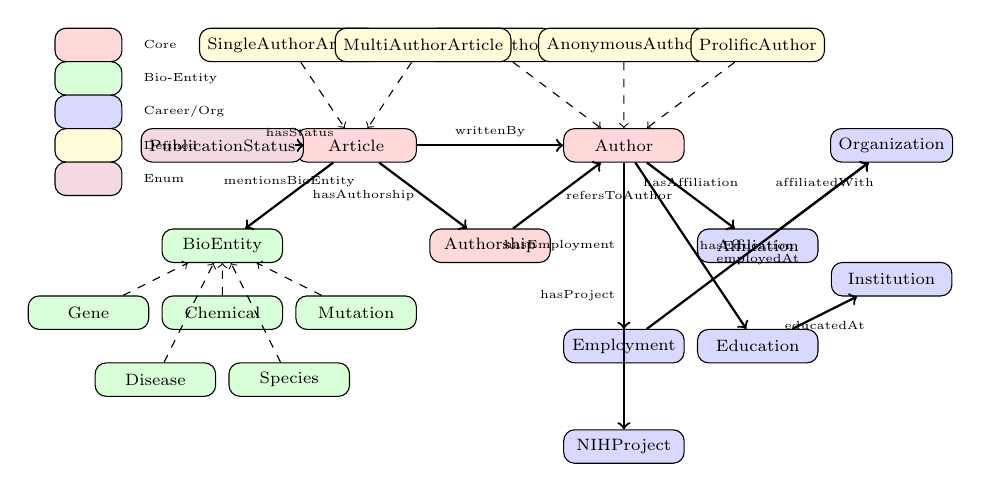
\begin{tikzpicture}[
    scale=0.85,
    transform shape,
    node distance=0.6cm,
    class/.style={draw, rounded corners, minimum width=1.8cm, minimum height=0.5cm, font=\scriptsize, align=center},
    core/.style={class, fill=red!15},
    bio/.style={class, fill=green!15},
    career/.style={class, fill=blue!15},
    defined/.style={class, fill=yellow!15},
    enum/.style={class, fill=purple!15},
    prop/.style={->, thick, font=\tiny}
]
    % === CORE CLASSES ===
    \node[core] (article) at (0,0) {Article};
    \node[core] (author) at (4,0) {Author};
    \node[core] (authorship) at (2,-1.5) {Authorship};
    
    % === ORGANIZATIONAL ===
    \node[career] (org) at (8,0) {Organization};
    \node[career] (inst) at (8,-2) {Institution};
    \node[career] (aff) at (6,-1.5) {Affiliation};
    
    % === CAREER ===
    \node[career] (emp) at (4,-3) {Employment};
    \node[career] (edu) at (6,-3) {Education};
    
    % === FUNDING ===
    \node[career] (nih) at (4,-4.5) {NIHProject};
    
    % === BIO-ENTITIES ===
    \node[bio] (bioent) at (-2,-1.5) {BioEntity};
    \node[bio] (gene) at (-4,-2.5) {Gene};
    \node[bio] (disease) at (-3,-3.5) {Disease};
    \node[bio] (chemical) at (-2,-2.5) {Chemical};
    \node[bio] (species) at (-1,-3.5) {Species};
    \node[bio] (mutation) at (0,-2.5) {Mutation};
    
    % === DEFINED CLASSES ===
    \node[defined] (active) at (2,1.5) {ActiveAuthor};
    \node[defined] (anon) at (4,1.5) {AnonymousAuthor};
    \node[defined] (prolific) at (6,1.5) {ProlificAuthor};
    \node[defined] (single) at (-1,1.5) {SingleAuthorArticle};
    \node[defined] (multi) at (1,1.5) {MultiAuthorArticle};
    
    % === ENUMERATION ===
    \node[enum] (status) at (-2,0) {PublicationStatus};
    
    % === RELATIONSHIPS ===
    \draw[prop] (article) -- node[above] {writtenBy} (author);
    \draw[prop] (article) -- node[left] {hasAuthorship} (authorship);
    \draw[prop] (authorship) -- node[right] {refersToAuthor} (author);
    \draw[prop] (article) -- node[above] {mentionsBioEntity} (bioent);
    \draw[prop] (article) -- node[above] {hasStatus} (status);
    
    \draw[prop] (author) -- node[above] {hasAffiliation} (aff);
    \draw[prop] (aff) -- node[above] {affiliatedWith} (org);
    \draw[prop] (author) -- node[left] {hasEmployment} (emp);
    \draw[prop] (emp) -- node[below] {employedAt} (org);
    \draw[prop] (author) -- node[right] {hasEducation} (edu);
    \draw[prop] (edu) -- node[below] {educatedAt} (inst);
    \draw[prop] (author) -- node[left] {hasProject} (nih);
    
    % Subclass arrows
    \draw[->, dashed] (gene) -- (bioent);
    \draw[->, dashed] (disease) -- (bioent);
    \draw[->, dashed] (chemical) -- (bioent);
    \draw[->, dashed] (species) -- (bioent);
    \draw[->, dashed] (mutation) -- (bioent);
    
    \draw[->, dashed] (active) -- (author);
    \draw[->, dashed] (anon) -- (author);
    \draw[->, dashed] (prolific) -- (author);
    \draw[->, dashed] (single) -- (article);
    \draw[->, dashed] (multi) -- (article);
    
    % Legend
    \node[core, minimum width=1cm] at (-4,1.5) {};
    \node[right, font=\tiny] at (-3.3,1.5) {Core};
    \node[bio, minimum width=1cm] at (-4,1) {};
    \node[right, font=\tiny] at (-3.3,1) {Bio-Entity};
    \node[career, minimum width=1cm] at (-4,0.5) {};
    \node[right, font=\tiny] at (-3.3,0.5) {Career/Org};
    \node[defined, minimum width=1cm] at (-4,0) {};
    \node[right, font=\tiny] at (-3.3,0) {Defined};
    \node[enum, minimum width=1cm] at (-4,-0.5) {};
    \node[right, font=\tiny] at (-3.3,-0.5) {Enum};
    
\end{tikzpicture}
\caption{Complete PKG2020 Ontology Schema with 23 Classes and Object Properties}
\label{fig:full-ontology}
\end{figure}

\subsection{RDF Triple Pattern (Subject-Predicate-Object)}

Figure \ref{fig:rdf-triple} illustrates the RDF triple pattern used throughout our knowledge graph.

\begin{figure}[H]
\centering
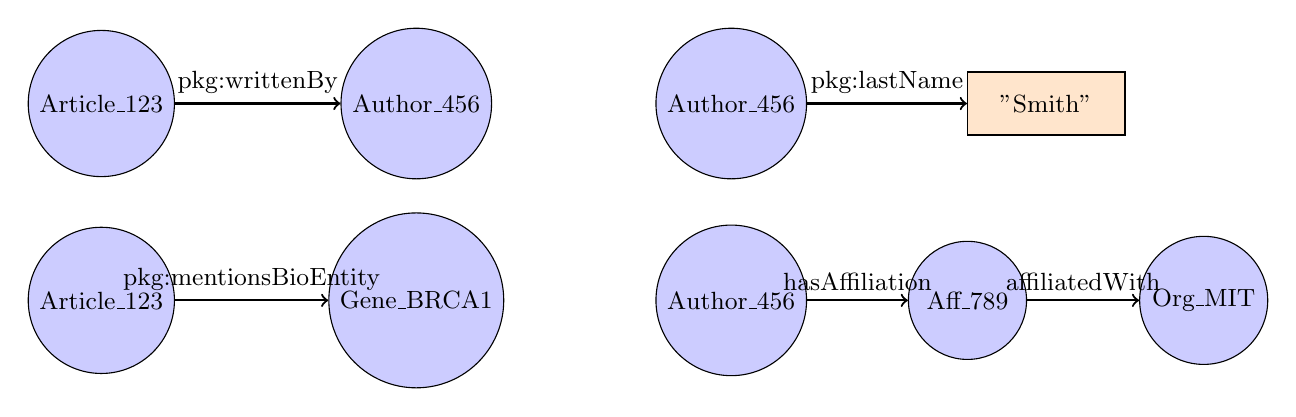
\begin{tikzpicture}[
    node distance=3cm,
    entity/.style={draw, circle, fill=blue!20, minimum size=1.5cm, font=\small},
    literal/.style={draw, rectangle, fill=orange!20, minimum width=2cm, minimum height=0.8cm, font=\small},
    pred/.style={->, thick, font=\small}
]
    % Example 1: Article -> writtenBy -> Author
    \node[entity] (art1) at (0,0) {Article\_123};
    \node[entity] (auth1) at (4,0) {Author\_456};
    \draw[pred] (art1) -- node[above] {pkg:writtenBy} (auth1);
    
    % Example 2: Author -> lastName -> "Smith"
    \node[entity] (auth2) at (8,0) {Author\_456};
    \node[literal] (name) at (12,0) {"Smith"};
    \draw[pred] (auth2) -- node[above] {pkg:lastName} (name);
    
    % Example 3: Article -> mentionsBioEntity -> Gene
    \node[entity] (art2) at (0,-2.5) {Article\_123};
    \node[entity] (gene1) at (4,-2.5) {Gene\_BRCA1};
    \draw[pred] (art2) -- node[above] {pkg:mentionsBioEntity} (gene1);
    
    % Example 4: Author -> hasAffiliation -> Affiliation -> affiliatedWith -> Org
    \node[entity] (auth3) at (8,-2.5) {Author\_456};
    \node[entity] (aff1) at (11,-2.5) {Aff\_789};
    \node[entity] (org1) at (14,-2.5) {Org\_MIT};
    \draw[pred] (auth3) -- node[above] {hasAffiliation} (aff1);
    \draw[pred] (aff1) -- node[above] {affiliatedWith} (org1);
    
\end{tikzpicture}
\caption{RDF Triple Pattern Examples: Subject $\rightarrow$ Predicate $\rightarrow$ Object}
\label{fig:rdf-triple}
\end{figure}

\subsection{Sample Knowledge Graph Visualization}

Figure \ref{fig:sample-kg} shows a sample subgraph from our knowledge graph demonstrating the interconnected nature of the data.

\begin{figure}[H]
\centering
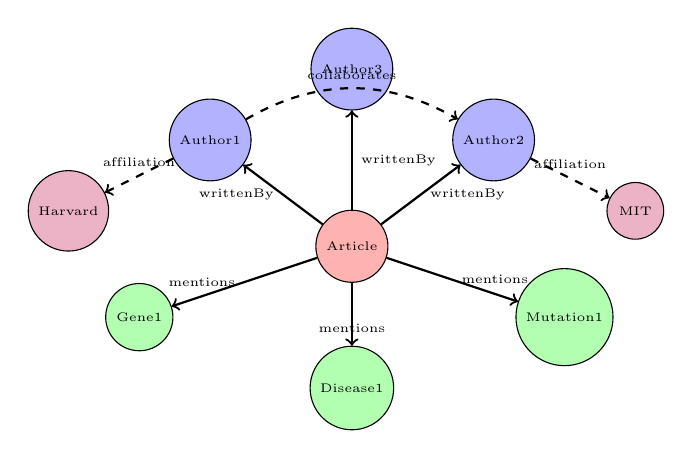
\begin{tikzpicture}[
    scale=0.9,
    transform shape,
    node distance=1.5cm,
    article/.style={draw, circle, fill=red!30, minimum size=1cm, font=\tiny},
    author/.style={draw, circle, fill=blue!30, minimum size=1cm, font=\tiny},
    bio/.style={draw, circle, fill=green!30, minimum size=0.8cm, font=\tiny},
    org/.style={draw, circle, fill=purple!30, minimum size=0.8cm, font=\tiny},
    edge/.style={->, thick, font=\tiny}
]
    % Central article
    \node[article] (art) at (0,0) {Article};
    
    % Authors
    \node[author] (a1) at (-2,1.5) {Author1};
    \node[author] (a2) at (2,1.5) {Author2};
    \node[author] (a3) at (0,2.5) {Author3};
    
    % Bio-entities
    \node[bio] (g1) at (-3,-1) {Gene1};
    \node[bio] (d1) at (0,-2) {Disease1};
    \node[bio] (m1) at (3,-1) {Mutation1};
    
    % Organizations
    \node[org] (o1) at (-4,0.5) {Harvard};
    \node[org] (o2) at (4,0.5) {MIT};
    
    % Article relationships
    \draw[edge] (art) -- node[left] {writtenBy} (a1);
    \draw[edge] (art) -- node[right] {writtenBy} (a2);
    \draw[edge] (art) -- node[right] {writtenBy} (a3);
    \draw[edge] (art) -- node[left] {mentions} (g1);
    \draw[edge] (art) -- node[below] {mentions} (d1);
    \draw[edge] (art) -- node[right] {mentions} (m1);
    
    % Author relationships
    \draw[edge, dashed] (a1) -- node[above] {affiliation} (o1);
    \draw[edge, dashed] (a2) -- node[above] {affiliation} (o2);
    \draw[edge, dashed, bend left] (a1) to node[above] {collaborates} (a2);
    
\end{tikzpicture}
\caption{Sample Knowledge Graph: Article with Authors, Bio-Entities, and Affiliations}
\label{fig:sample-kg}
\end{figure}

\subsection{Knowledge Graph Statistics}

\begin{figure}[H]
\centering
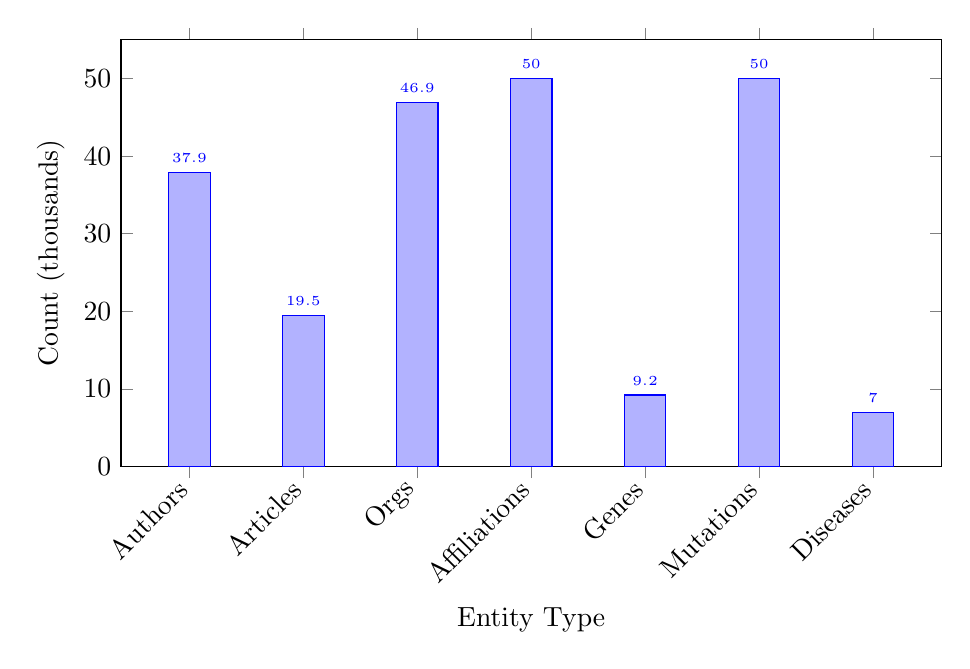
\begin{tikzpicture}
    \begin{axis}[
        ybar,
        bar width=15pt,
        width=12cm,
        height=7cm,
        xlabel={Entity Type},
        ylabel={Count (thousands)},
        symbolic x coords={Authors, Articles, Orgs, Affiliations, Genes, Mutations, Diseases},
        xtick=data,
        x tick label style={rotate=45, anchor=east},
        ymin=0,
        nodes near coords,
        nodes near coords style={font=\tiny},
        every axis plot/.append style={fill=blue!30}
    ]
    \addplot coordinates {
        (Authors, 37.9)
        (Articles, 19.5)
        (Orgs, 46.9)
        (Affiliations, 50.0)
        (Genes, 9.2)
        (Mutations, 50.0)
        (Diseases, 7.0)
    };
    \end{axis}
\end{tikzpicture}
\caption{Distribution of Entity Types in Knowledge Graph (2.1M+ triples)}
\label{fig:entity-stats}
\end{figure}

\subsection{Tools Used}

\begin{itemize}
    \item \textbf{Protégé}: Desktop ontology editor and visualizer
    \item \textbf{GraphDB Sandbox}: Cloud-hosted triple store with SPARQL endpoint
    \item \textbf{WebVOWL}: Online ontology visualization
    \item \textbf{Custom Flask App}: Interactive web-based explorer with D3.js graphs
\end{itemize}

\subsection{Web Application Features}

Our Flask-based web application provides:

\begin{enumerate}
    \item \textbf{Dashboard}: Real-time statistics fetched from GraphDB
    \item \textbf{Live KG Explorer}: Interactive D3.js force-directed graph visualization
    \item \textbf{SPARQL Query Editor}: Execute queries with Table/Graph/Chart views
    \item \textbf{12 Competency Queries}: Pre-built queries for common questions
\end{enumerate}

\begin{figure}[H]
\centering
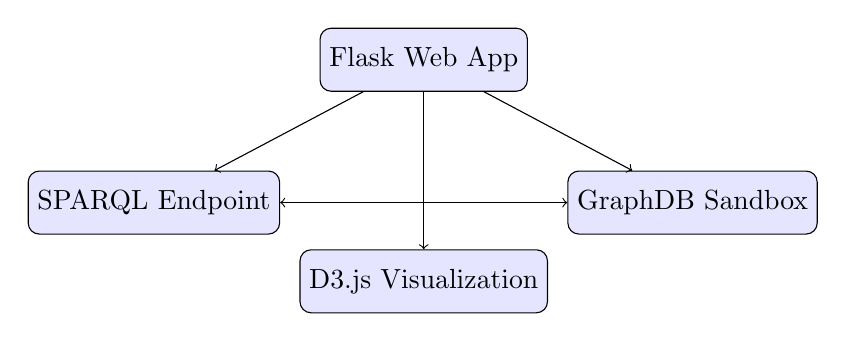
\begin{tikzpicture}[
    node distance=1cm,
    box/.style={draw, rounded corners, minimum width=2.5cm, minimum height=0.8cm, fill=blue!10}
]
    \node[box] (webapp) {Flask Web App};
    \node[box, below left=1cm and 0.5cm of webapp] (sparql) {SPARQL Endpoint};
    \node[box, below right=1cm and 0.5cm of webapp] (graphdb) {GraphDB Sandbox};
    \node[box, below=2cm of webapp] (d3) {D3.js Visualization};
    
    \draw[->] (webapp) -- (sparql);
    \draw[->] (webapp) -- (graphdb);
    \draw[->] (webapp) -- (d3);
    \draw[<->] (sparql) -- (graphdb);
\end{tikzpicture}
\caption{Web Application Architecture}
\label{fig:webapp-arch}
\end{figure}

\subsection{Live GraphDB Endpoint}

Our knowledge graph is accessible via the public SPARQL endpoint:

\begin{verbatim}
https://x1327f4041a654297998.sandbox.graphwise.ai
    /repositories/KRR-Project
\end{verbatim}

\textbf{Statistics:}
\begin{itemize}
    \item 2,165,964 total triples
    \item 23 ontology classes
    \item 14 object properties
    \item 17+ data properties
\end{itemize}

%==============================================================================
\section{Reflection}
%==============================================================================

\subsection{Learning Outcomes}

Through this project, we learned:

\begin{enumerate}
    \item How to design ontologies following OWL/RDF standards
    \item The importance of defined classes for reasoning
    \item How to link data to external knowledge bases
    \item The power of SPARQL for semantic querying
    \item Practical application of knowledge representation concepts
\end{enumerate}

\subsection{Added Value of Linked Data}

Converting non-RDF data to linked data enabled:

\begin{itemize}
    \item Semantic querying across heterogeneous datasets
    \item Reasoning over implicit relationships
    \item Integration with global knowledge bases (DBpedia, Wikidata)
    \item FAIR data principles compliance
    \item Interoperability with other linked data systems
\end{itemize}

\subsection{Challenges Faced}

\begin{enumerate}
    \item Large file sizes required memory optimization
    \item Special characters in organization names caused parsing issues
    \item Reasoner installation and configuration
    \item Balancing between sample size and processing time
\end{enumerate}

%==============================================================================
\section{Conclusion}
%==============================================================================

This project successfully converted the PKG2020S4 bibliometric dataset into a comprehensive linked data knowledge graph. We achieved:

\begin{enumerate}
    \item \textbf{Ontology Design}: 20+ classes with all required axioms
    \item \textbf{Data Population}: Modular Python pipeline for 7 CSV files
    \item \textbf{Reasoning}: Consistency checking and classification
    \item \textbf{External Linking}: 5-star linked data with DBpedia/Wikidata
    \item \textbf{SPARQL Queries}: 15 competency questions answered
    \item \textbf{Web Application}: Interactive web application for exploring the knowledge graph
\end{enumerate}

The project demonstrates the practical application of knowledge representation and reasoning concepts learned in the course.

%==============================================================================
\section{References}
%==============================================================================

\begin{enumerate}
    \item Lamy, J. B. (2017). OWLReady: Ontology-oriented programming in Python. Artificial Intelligence in Medicine.
    \item W3C. (2012). OWL 2 Web Ontology Language Primer.
    \item DBpedia Association. (2024). DBpedia Knowledge Base.
    \item PubMed. (2024). NCBI PubMed Database.
\end{enumerate}

%==============================================================================
\section{Appendix: Project Repository}
%==============================================================================

The complete project code is available at:

\url{https://github.com/Zain-Haider-ai-63/Knowlege-Graphs-Project}

\subsection{Repository Structure}

\begin{lstlisting}
Knowledge_Graphs_Project/
+-- scripts/           # Python scripts
+-- owl/               # Generated OWL files
+-- docs/              # Documentation
+-- requirements.txt   # Dependencies
+-- README.md          # Project overview
\end{lstlisting}

\end{document}
